% ----------------------------------------------------------------------------
%                                  RESULTADOS
% ----------------------------------------------------------------------------

\chapter{METODOLOGIA}
\label{chap:metodologia}

Este capítulo detalha as etapas de planejamento, construção e validação da transição do Painel Parkinson para o ambiente \textit{desktop}, apresentando desde o cronograma de execução até as análises preliminares de usabilidade.

\section{Classificação da Pesquisa}
\label{sec:classificacao_pesquisa}

A pesquisa científica consiste em um processo sistemático que busca construir novos conhecimentos ou técnicas para explicar fenômenos e solucionar problemas cotidianos \cite{santos2021metodologia}. Para o desenvolvimento deste trabalho, o percurso metodológico foi estruturado com base nas classificações clássicas das ciências, considerando a sua natureza, abordagem, objetivos e procedimentos técnicos \cite{fonseca2023tipos} e \cite{santos2021metodologia}.

Quanto à sua natureza, esta investigação classifica-se como pesquisa aplicada \cite{santos2021metodologia}, pois possui como objetivo o desenvolvimento de uma solução computacional voltada ao apoio clínico no acompanhamento de pacientes diagnosticados com Doença de Parkinson. Esse tipo de estudo tem como finalidade a produção de novos conhecimentos, processos ou tecnologias que possuam aplicação prática e imediata.

Quanto à abordagem, a pesquisa adota uma perspectiva mista, de caráter qualitativo e quantitativo \cite{santos2021metodologia}. O aspecto qualitativo está relacionado à avaliação da experiência dos profissionais da saúde durante a utilização do sistema, considerando fatores como usabilidade, acessibilidade e organização visual da interface. Já o aspecto quantitativo envolve a coleta de métricas e a análise de desempenho da aplicação, o tempo de resposta, a estabilidade do sistema e o processamento das informações clínicas.

Em relação aos objetivos, o estudo enquadra-se metodologicamente como uma pesquisa exploratória e descritiva \cite{santos2021metodologia}. A etapa exploratória busca compreender tecnologias, arquiteturas e abordagens utilizadas em sistemas de apoio à decisão clínica. Simultaneamente, a pesquisa possui caráter descritivo por observar, analisar e documentar as características estruturais, funcionais e visuais da aplicação desenvolvida.

Por fim, quanto aos procedimentos técnicos, a pesquisa fundamenta-se na revisão bibliográfica, no mapeamento sistemático da literatura e no desenvolvimento experimental \cite{santos2021metodologia}. A revisão e o mapeamento sistemático foram utilizados para identificar trabalhos relacionados e lacunas tecnológicas. O desenvolvimento experimental ocorreu por meio da adaptação do Painel Parkinson para o ambiente \textit{desktop}, utilizando tecnologias como Electron.js, VueJS, Python e PostgreSQL. Além disso, a pesquisa incorpora testes preliminares com potenciais usuários para buscar evidências práticas do desempenho da solução no contexto clínico.

\section{Modelagem Funcional do Sistema}
\label{sec:modelagem_funcional}

Esta seção apresenta a modelagem funcional da aplicação \textit{desktop}, mapeando as interações dos usuários com o sistema e o comportamento dos fluxos de dados internos através de diagramas da \textit{Unified Modeling Language} (UML). Para a estruturação e geração visual dos diagramas apresentados nesta seção, utilizou-se a linguagem e ferramenta de código aberto PlantUML.

\subsection{Diagrama de Casos de Uso}
O Diagrama de Casos de Uso, apresentado na Figura~\ref{fig:casos_de_uso}, delimita o escopo do sistema e as ações que o profissional de saúde pode executar na interface local. 

\begin{figure}[htb]
    \centering
    \caption{Diagrama de Casos de Uso do Painel Parkinson \textit{Desktop}.}
    \label{fig:casos_de_uso}
    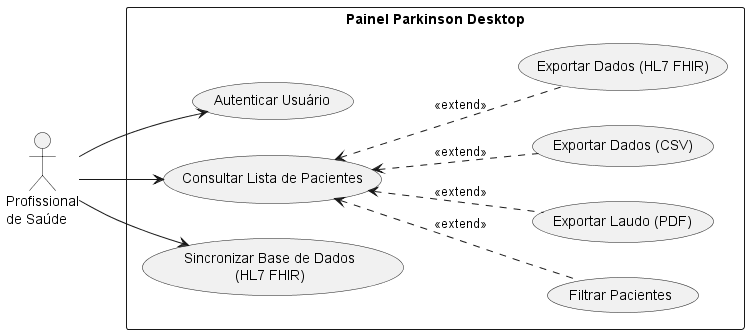
\includegraphics[width=0.7\textwidth]{caso_de_uso_painelParkinson.png}
    \centerline{\footnotesize Fonte: Elaborado pelos autores (2026).}
\end{figure}

A partir da modelagem, observa-se que o ator principal (Profissional de Saúde) interage diretamente com as rotinas de consulta, filtragem e exportação de dados clínicos, disponibilizadas em formatos versáteis como PDF para laudos, CSV para análises tabulares e o padrão global \textbf{HL7 FHIR} para interoperabilidade estruturada. Adicionalmente, o diagrama evidencia o fluxo de sincronização baseado no protocolo \textbf{HL7 FHIR} com o repositório central SIDABI, assegurando que a persistência local, a conformidade com a LGPD através da anonimação e a troca segura de informações ocorram de forma transparente e padronizada.

\subsection{Diagrama de Sequência}
Para detalhar a comunicação assíncrona entre os componentes da arquitetura \textit{desktop}, a Figura~\ref{fig:diagrama_sequencia} ilustra o Diagrama de Sequência para a renderização de um relatório clínico, evidenciando o papel do Electron.js como intermediador de chamadas.

\begin{figure}[H]
    \centering
    \caption{Diagrama de Sequência para carregamento de painéis biomédicos.}
    \label{fig:diagrama_sequencia}
    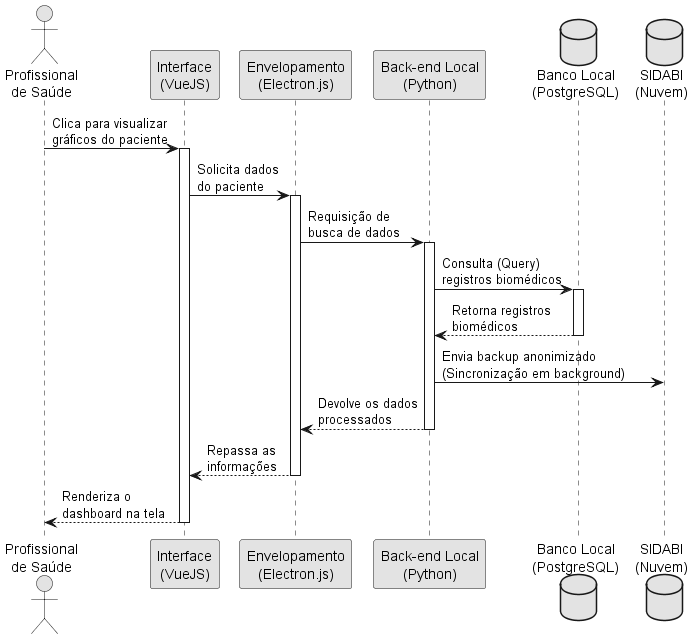
\includegraphics[width=0.8\textwidth]{diagrama_sequencia_PainelParkinson.png}
    \centerline{\footnotesize Fonte: Elaborado pelos autores (2026).}
\end{figure}

\section{Arquitetura da Solução e Integração Tecnológica}
\label{sec:arquitetura_solucao}

A transição do modelo arquitetural web para uma topologia \textit{desktop} exige o isolamento de componentes para assegurar baixa latência no processamento gráfico e viabilizar a redução de custos de infraestrutura em nuvem. A Figura~\ref{fig:arquitetura_blocos} apresenta a visão macroscópica da distribuição dos módulos do sistema.

\begin{figure}[H]
    \centering
    \caption{Diagrama da Arquitetura em camadas da aplicação \textit{desktop}.}
    \label{fig:arquitetura_blocos}
    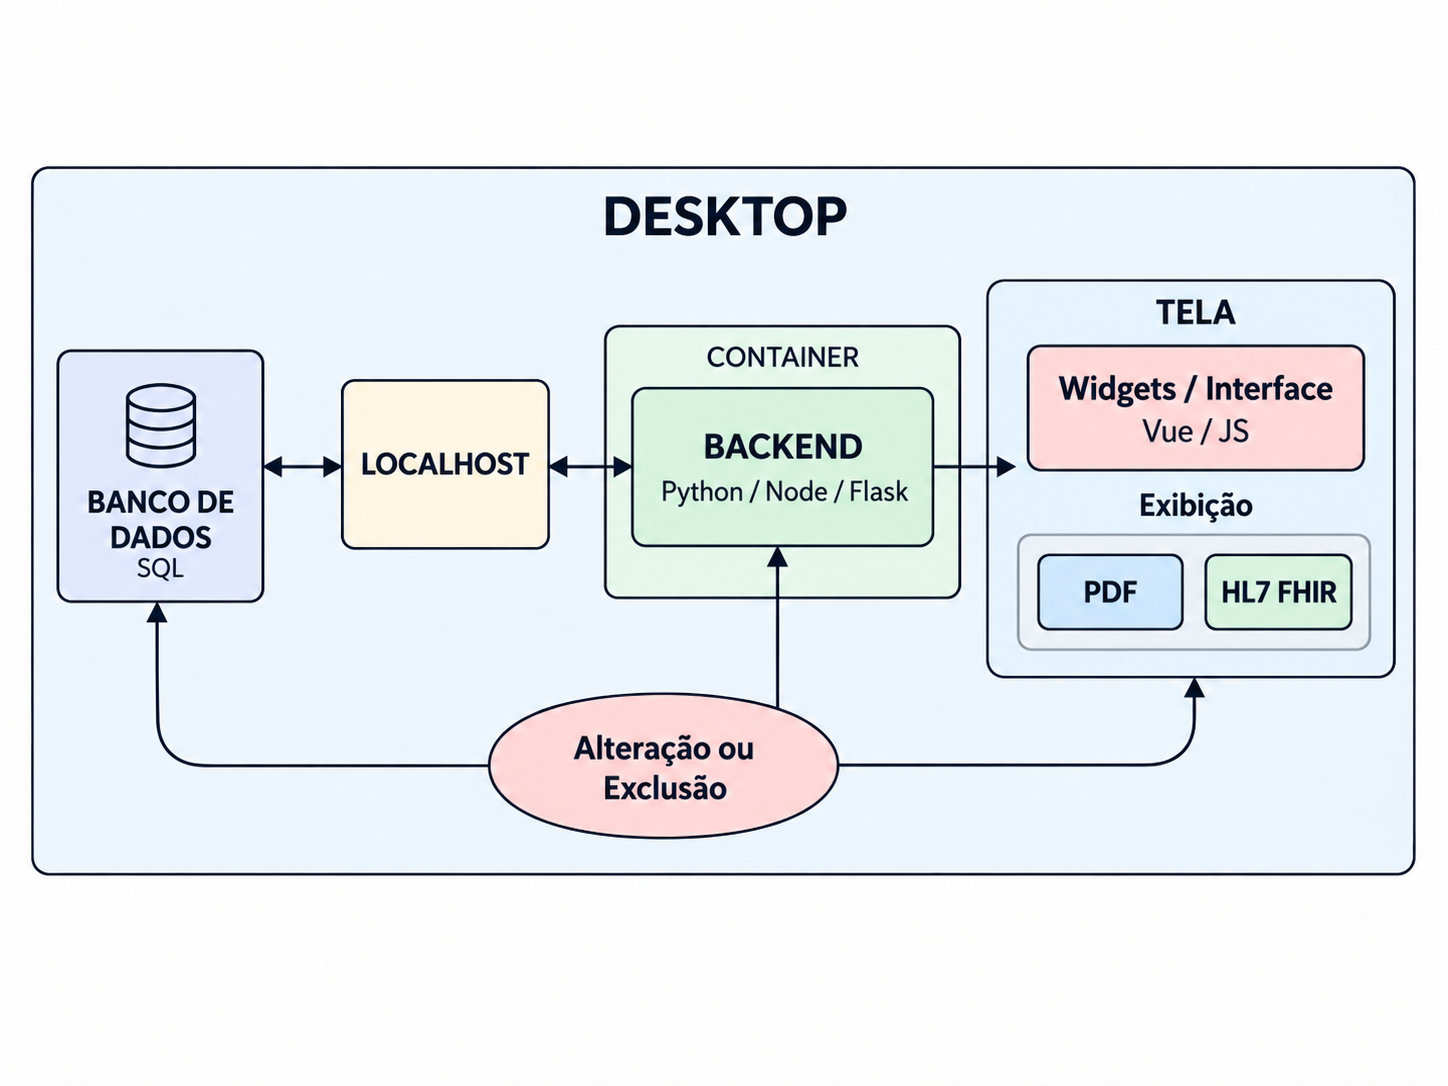
\includegraphics[width=0.8\textwidth]{arquitetura_painelParkinson.png}
    \centerline{\footnotesize Fonte: Elaborado pelos autores (2026).}
\end{figure}

Conforme ilustrado na Figura~\ref{fig:arquitetura_blocos}, a arquitetura reúne o banco de dados, a comunicação local, o processamento e a interface no ambiente \textit{desktop}. O diagrama também apresenta as opções de exportação dos dados do paciente e o fluxo de alteração ou exclusão dos registros:

\begin{itemize}
    \item \textbf{Banco de dados e comunicação local:} O banco de dados SQL armazena os registros utilizados no acompanhamento dos pacientes. A comunicação com os serviços ocorre no ambiente local, indicado no diagrama pelo endereço \textit{localhost}.

    \item \textbf{Processamento e serviços:} O \textit{back-end}, representado no contêiner, recebe as solicitações da aplicação, realiza o tratamento dos dados e interage com o banco. O diagrama identifica Python, Node.js e Flask como tecnologias relacionadas ao ambiente de execução e aos serviços.

    \item \textbf{Interface e apresentação:} A tela, construída com Vue e JavaScript, organiza os componentes visuais e apresenta os dados clínicos nos painéis informativos, permitindo ao profissional consultar as informações do paciente.

    \item \textbf{Exportação dos dados do paciente:} A interface oferece a escolha entre PDF e HL7 FHIR. O PDF apresenta um relatório destinado à leitura e impressão, enquanto a opção FHIR permite exportar informações estruturadas para intercâmbio com sistemas de saúde compatíveis, conforme discutido na Seção~\ref{sec:hl7-fhir}.

    \item \textbf{Alteração e exclusão:} O fluxo indicado na parte inferior do diagrama relaciona essas operações ao processamento, à persistência e à apresentação. As alterações nos registros devem ser refletidas no banco de dados e na interface para manter a consistência das informações exibidas.
\end{itemize}

\section{Regras de Negócio e Especificação de Requisitos}
\label{sec:requisitos_regras}

Para garantir que a arquitetura \textit{desktop} atenda às necessidades clínicas de acompanhamento da Doença de Parkinson e respeite as diretrizes de engenharia de \textbf{software}, o sistema foi documentado através de Regras de Negócio (RN), Requisitos Funcionais (RF) e Requisitos Não Funcionais (RNF).

\subsection{Regras de Negócio (RN)}
As Regras de Negócio definem as políticas, restrições e condições lógicas que orientam o comportamento do Painel Parkinson, garantindo a segurança e a validade dos dados em ambiente médico. O Quadro~\ref{quadro:rn01} e o Quadro~\ref{quadro:rn02} detalham as principais restrições do sistema.

\begin{quadro}[htb]
\centering
\caption{Especificação da Regra de Negócio 01 (RN01) - Controle de Acesso}
\label{quadro:rn01}
\begin{tabular}{|l|p{11cm}|}
\hline
\textbf{Identificador} & \textbf{RN01} \\ \hline
\textbf{Nome} & Restrição de Acesso Clínico \\ \hline
\textbf{Descrição} & O acesso aos dados e aos painéis analíticos dos pacientes só pode ser realizado por profissionais de saúde previamente autenticados e vinculados ao sistema, visando a proteção de dados sensíveis. \\ \hline
\textbf{Restrição} & Impede visualização anônima ou pública. \\ \hline
\end{tabular}
\centerline{\footnotesize Fonte: Elaborado pelos autores (2026).}
\end{quadro}

\begin{quadro}[htb]
\centering
\caption{Especificação da Regra de Negócio 02 (RN02) - Integridade da Origem}
\label{quadro:rn02}
\begin{tabular}{|l|p{11cm}|}
\hline
\textbf{Identificador} & \textbf{RN02} \\ \hline
\textbf{Nome} & Leitura de Dados do SIDABI \\ \hline
\textbf{Descrição} & O Painel Parkinson atua primordialmente como uma ferramenta de visualização e apoio à decisão. Os dados primários provenientes do banco de dados SIDABI não devem sofrer mutações estruturais através da interface \textit{desktop}, garantindo a integridade histórica da pesquisa. \\ \hline
\textbf{Restrição} & Bloqueio de exclusão em massa de registros biomédicos. \\ \hline
\end{tabular}
\centerline{\footnotesize Fonte: Elaborado pelos autores (2026).}
\end{quadro}

\begin{quadro}[htb]
\centering
\caption{Especificação da Regra de Negócio 03 (RN03) - Anonimização em Exportações}
\label{quadro:rn03}
\begin{tabular}{|l|p{11cm}|}
\hline
\textbf{Identificador} & \textbf{RN03} \\ \hline
\textbf{Nome} & Anonimização Obrigatória em Exportações de Lote \\ \hline
\textbf{Descrição} & A exportação de dados gerais do sistema para o formato CSV deve obrigatoriamente omitir ou mascarar dados sensíveis de identificação direta do paciente. \\ \hline
\textbf{Restrição} & O sistema deve gerar um identificador único (ID/Hash) para cada paciente no arquivo exportado, permitindo o uso dos dados biométricos e clínicos para pesquisa científica sem expor a identidade real dos indivíduos. \\ \hline
\end{tabular}
\centerline{\footnotesize Fonte: Elaborado pelos autores (2026).}
\end{quadro}

\subsection{Requisitos Funcionais (RF)}
Os Requisitos Funcionais descrevem as ações e funcionalidades diretas que a aplicação deve oferecer aos usuários durante a sua execução. Os quadros a seguir apresentam os cartões de especificação das principais funções do sistema local.

\begin{quadro}[H]
\centering
\caption{Especificação do Requisito Funcional 01 (RF01) - Renderização de Gráficos}
\label{quadro:rf01}
\begin{tabular}{|l|p{11cm}|}
\hline
\textbf{Identificador} & \textbf{RF01} \\ \hline
\textbf{Nome} & Renderização de \textit{Dashboards} Clínicos \\ \hline
\textbf{Descrição} & O sistema deve exibir gráficos iterativos no \textit{front-end} em VueJS, representando a evolução motora e os dados dos pacientes diagnosticados com a Doença de Parkinson de forma clara. \\ \hline
\textbf{Prioridade} & Alta \\ \hline
\textbf{Ator} & Profissional de Saúde / Médico \\ \hline
\end{tabular}
\centerline{\footnotesize Fonte: Elaborado pelos autores (2026).}
\end{quadro}

\begin{quadro}[H]
\centering
\caption{Especificação do Requisito Funcional 02 (RF02) - Exportação de Dados}
\label{quadro:rf02}
\begin{tabular}{|l|p{11cm}|}
\hline
\textbf{Identificador} & \textbf{RF02} \\ \hline
\textbf{Nome} & Geração de Laudo Clínico Individual (PDF) \\ \hline
\textbf{Descrição} & O sistema deve permitir que o profissional de saúde gere e faça o \textit{download} de um laudo individualizado do paciente atual em formato PDF, consolidando as informações da escala MDS-UPDRS para entrega ao paciente ou anexação ao prontuário físico. \\ \hline
\textbf{Prioridade} & Média \\ \hline
\textbf{Ator} & Profissional de Saúde / Médico \\ \hline
\end{tabular}
\centerline{\footnotesize Fonte: Elaborado pelos autores (2026).}
\end{quadro}

\begin{quadro}[H]
\centering
\caption{Especificação do Requisito Funcional 03 (RF03) - Filtragem Dinâmica}
\label{quadro:rf03}
\begin{tabular}{|l|p{11cm}|}
\hline
\textbf{Identificador} & \textbf{RF03} \\ \hline
\textbf{Nome} & Filtragem Dinâmica de Dados Clínicos \\ \hline
\textbf{Descrição} & O sistema deve disponibilizar filtros iterativos para que o profissional de saúde isole períodos específicos ou variáveis biomotoras isoladas nos painéis de visualização. \\ \hline
\textbf{Prioridade} & Alta \\ \hline
\textbf{Ator} & Profissional de Saúde / Médico \\ \hline
\end{tabular}
\centerline{\footnotesize Fonte: Elaborado pelos autores (2026).}
\end{quadro}

\begin{quadro}[H]
\centering
\caption{Especificação do Requisito Funcional 04 (RF04) - Sincronização Automática em Background}
\label{quadro:rf04}
\begin{tabular}{|l|p{11cm}|}
\hline
\textbf{Identificador} & \textbf{RF04} \\ \hline
\textbf{Nome} & Sincronização Automática em Background \\ \hline
\textbf{Descrição} & O sistema deve realizar automaticamente, em segundo plano (\textit{background}), a sincronização dos dados clínicos anonimizados armazenados localmente com a base de dados de pesquisa do SIDABI, mantendo o histórico biomédico atualizado durante a utilização da aplicação. Como mecanismo de contingência, a aplicação poderá disponibilizar uma opção de sincronização manual para situações excepcionais. \\ \hline
\textbf{Prioridade} & Alta \\ \hline
\textbf{Ator} & Sistema \\ \hline
\end{tabular}
\centerline{\footnotesize Fonte: Elaborado pelos autores (2026).}
\end{quadro}

\begin{quadro}[H]
\centering
\caption{Especificação do Requisito Funcional 05 (RF05) - Exportação de Dados em Lote}
\label{quadro:rf05}
\begin{tabular}{|l|p{11cm}|}
\hline
\textbf{Identificador} & \textbf{RF05} \\ \hline
\textbf{Nome} & Exportação de Dados em Lote para Pesquisa (CSV) \\ \hline
\textbf{Descrição} & \raggedright O sistema deve fornecer uma funcionalidade para que qualquer profissional de saúde autenticado realize o \textit{download} de toda a base de dados local em formato CSV, aplicando automaticamente as regras de anonimização (RN03) para viabilizar análises estatísticas em ferramentas externas. \tabularnewline \hline
\textbf{Prioridade} & Média \\ \hline
\textbf{Ator} & Profissional de Saúde \\ \hline
\end{tabular}
\centerline{\footnotesize Fonte: Elaborado pelos autores (2026).}
\end{quadro}

\subsection{Requisitos Não Funcionais (RNF)}
Os Requisitos Não Funcionais especificam as restrições tecnológicas, os critérios de desempenho e os quesitos de infraestrutura que qualificam a operação do software desenvolvido.

\begin{quadro}[H]
\centering
\caption{Especificação do Requisito Não Funcional 01 (RNF01) - Desempenho Local}
\label{quadro:rnf01}
\begin{tabular}{|l|p{11cm}|}
\hline
\textbf{Identificador} & \textbf{RNF01} \\ \hline
\textbf{Nome} & Baixa Latência de Processamento \\ \hline
\textbf{Descrição} & A comunicação entre o \textit{front-end} envelopado pelo Electron e o \textit{back-end} em Python deve ocorrer no ambiente local, minimizando a latência na renderização dos dados. Além disso, a sincronização automática dos dados em segundo plano (\textit{background}) deve ocorrer sem comprometer a responsividade da interface durante a utilização da aplicação. \\ \hline
\textbf{Prioridade} & Alta \\ \hline
\textbf{Categoria} & Desempenho / Arquitetura \\ \hline
\end{tabular}
\centerline{\footnotesize Fonte: Elaborado pelos autores (2026).}
\end{quadro}

\begin{quadro}[H]
\centering
\caption{Especificação do Requisito Não Funcional 02 (RNF02) - Otimização de Custos}
\label{quadro:rnf02}
\begin{tabular}{|l|p{11cm}|}
\hline
\textbf{Identificador} & \textbf{RNF02} \\ \hline
\textbf{Nome} & Independência de Hospedagem em Nuvem \\ \hline
\textbf{Descrição} & A arquitetura da solução deve ser majoritariamente descentralizada para a máquina do cliente, reduzindo os custos operacionais com servidores em nuvem para processamento contínuo da aplicação web original. \\ \hline
\textbf{Prioridade} & Alta \\ \hline
\textbf{Categoria} & Infraestrutura / Viabilidade \\ \hline
\end{tabular}
\centerline{\footnotesize Fonte: Elaborado pelos autores (2026).}
\end{quadro}

\begin{quadro}[H]
\centering
\caption{Especificação do Requisito Não Funcional 03 (RNF03) - Segurança e LGPD}
\label{quadro:rnf03}
\begin{tabular}{|l|p{11cm}|}
\hline
\textbf{Identificador} & \textbf{RNF03} \\ \hline
\textbf{Nome} & Segurança de Dados Sensíveis \\ \hline
\textbf{Descrição} & A aplicação deve trafegar os dados dos pacientes utilizando protocolos de criptografia, em conformidade com as diretrizes de privacidade da Lei Geral de Proteção de Dados (LGPD) para informações da área da saúde. Adicionalmente, a coleta e o envio de dados para o banco central do SIDABI devem ser condicionados ao aceite de um termo de consentimento, garantindo a prévia anonimização das informações sensíveis pelo sistema local. \\ \hline
\textbf{Prioridade} & Alta \\ \hline
\textbf{Categoria} & Segurança / Legal \\ \hline
\end{tabular}
\centerline{\footnotesize Fonte: Elaborado pelos autores (2026).}
\end{quadro}

\begin{quadro}[H]
\centering
\caption{Especificação do Requisito Não Funcional 04 (RNF04) - Consumo de Recursos}
\label{quadro:rnf04}
\begin{tabular}{|l|p{11cm}|}
\hline
\textbf{Identificador} & \textbf{RNF04} \\ \hline
\textbf{Nome} & Otimização de Memória RAM \\ \hline
\textbf{Descrição} & Devido ao encapsulamento via Electron.js, a aplicação deve implementar o gerenciamento eficiente de processos de renderização em segundo plano, evitando o consumo excessivo de memória RAM na máquina local. \\ \hline
\textbf{Prioridade} & Média \\ \hline
\textbf{Categoria} & Desempenho / Hardware \\ \hline
\end{tabular}
\centerline{\footnotesize Fonte: Elaborado pelos autores (2026).}
\end{quadro}


\section{Desenvolvimento e Interface}

\subsection{Desenvolvimento da Interface \textit{Desktop}}

Após a definição da arquitetura da solução, iniciou-se o processo de adaptação visual do Painel Parkinson para o ambiente \textit{desktop}. O objetivo principal dessa etapa foi proporcionar uma experiência de utilização mais prática, rápida e eficiente para profissionais da saúde durante o acompanhamento clínico de pacientes diagnosticados com a Doença de Parkinson.
A interface da aplicação foi mantida utilizando o \textit{framework} VueJS, preservando os componentes visuais já existentes na versão \textit{web} do sistema. Dessa forma, foi possível reutilizar os \textit{dashboards} clínicos, gráficos e estruturas de navegação desenvolvidas nas versões anteriores do Painel Parkinson, originalmente idealizado e desenvolvido por \cite{oliveira2021}, \cite{costa2022sistema} e \cite{oliveira2023}.

\subsubsection{Propostas de Aprimoramento e Funcionalidades Sugeridas}
\label{subsubsec:propostas_aprimoramento_sugeridas}

O estudo prévio de usabilidade conduzido por \cite{rabelo2025} mapeou uma série de falhas sistêmicas (IDPs) e oportunidades de melhoria na versão \textit{web} original do Painel Parkinson. Enquanto o referido trabalho limitou-se a catalogar e sugerir melhorias sob uma perspectiva conceitual, a presente migração arquitetural para o ambiente \textit{desktop} foi concebida especificamente para implementar, sanar e consolidar essas demandas na prática. 

A adoção do \textit{framework} Electron.js atuou como o alicerce definitivo para estas implementações. Ao unificar o \textit{front-end} reativo em VueJS com a capacidade de processamento local do Python (Flask) e o banco de dados PostgreSQL, os problemas de usabilidade listados na Seção 2.7.1 foram integralmente resolvidos pelas seguintes soluções de engenharia de \textit{software}:

\begin{enumerate}
    \item \textbf{Interface, Usabilidade e Navegação Estável (Mitigação dos IDP4, IDP6, IDP9 e IDP10):}
    \begin{itemize}
        \item \textit{Resolução do IDP4 (Botão Voltar):} A execução da aplicação dentro de uma janela nativa do Electron (\textit{BrowserWindow}) permitiu omitir as barras de navegação tradicionais de navegadores de \textit{internet}. A navegação interna é gerenciada de forma estrita pelo \textit{Vue Router} de forma programática. Isso elimina por completo o uso acidental do botão ``voltar'' do navegador pelo clínico, extinguindo os redirecionamentos cíclicos e a duplicação indesejada de históricos de navegação.
        \item \textit{Resolução do IDP6 (Visualização de Gráficos de Tremor):} Gráficos dinâmicos que sofriam congelamento ou perda de pontos de dados durante operações de \textit{zoom} foram reestruturados com bibliotecas de renderização assíncrona baseadas em Canvas e WebGL, rodando localmente na GPU da máquina cliente por meio do processo de renderização do Electron (\textit{Chromium Render Process}). O processamento local de vetores em Python elimina a latência de requisição de rede, garantindo que o carregamento do histórico longitudinal de avaliações clínicas (MDS-UPDRS) seja instantâneo, deixando a arquitetura já preparada para a futura reintrodução de gráficos com grande volume de dados.
        \item \textit{Resolução dos IDP9 e IDP10 (Interatividade e Scroll):} Elementos inativos ou em desenvolvimento que confundiam o clínico foram removidos ou receberam estados reativos de desabilitação condicional no VueJS (atributos \textit{:disabled}). Menus redundantes foram simplificados, e a barra de rolagem foi automatizada para acompanhar o foco visual do profissional de saúde durante preenchimentos de formulários clínicos, minimizando a carga cognitiva.
    \end{itemize}

    \item \textbf{Rigor Clínico e Persistência das Escalas MDS-UPDRS (Mitigação dos IDP1, IDP2, IDP5 e IDP8):}
    \begin{itemize}
        \item \textit{Resolução de IDP1, IDP2 e IDP5 (Perda de Filtros Clínicos):} Na versão \textit{web}, o recarregamento de páginas ou o trânsito entre telas limpava as seleções de condições críticas (como as subcondições clínicas ``com estímulo'' ou ``sem estímulo''). Na versão \textit{desktop}, o estado de seleção é gerenciado de forma persistente através de uma loja de estados centralizada no \textit{front-end} (Pinia/Vuex), que opcionalmente armazena os parâmetros temporais no banco PostgreSQL local. Com isso, os filtros permanecem intactos durante toda a sessão de análise do paciente.
        \item \textit{Resolução do IDP8 (Exibição de Dados Incorretos):} Para evitar o pré-carregamento de dados obsoletos na interface da UPDRS antes de validar a seleção, implementou-se um ciclo de vida de rotas no VueJS (\textit{navigation guards}). A tela é liberada para renderização apenas após o \textit{back-end} local em Flask disparar uma \textit{Promise}, confirmando a validação estrutural e a integridade da consulta SQL retornada pelo banco PostgreSQL local. Isso elimina o risco de indução ao erro médico.
        \item \textit{Nomenclatura e Cálculos Clínicos:} Toda a interface de escalas foi atualizada para adotar a nomenclatura oficial regulamentada pela \textit{International Parkinson and Movement Disorder Society} (MDS-UPDRS). Adicionalmente, a aplicação automatiza os cálculos de soma dos escores de cada domínio clínico (Partes I, II, III e IV) em tempo real, gerando relatórios dinâmicos.
    \end{itemize}

    \item \textbf{Privacidade dos Dados Clínicos e Sincronização Inteligente em Background (RF04 / RNF03):}
    \begin{itemize}
        \item Para garantir estrita conformidade com a Lei Geral de Proteção de Dados (LGPD) no manuseio de dados de saúde sensíveis, a arquitetura local isola as informações de identificação direta do paciente no PostgreSQL instalado localmente na instituição de saúde. 
        \item A comunicação com a base de dados central de pesquisa SIDABI \cite{folador2021} é efetuada de forma segura e automatizada em segundo plano (\textit{background}) pelo Electron. O sistema realiza um processo de anonimização (em conformidade com o Art. 13 da Lei nº 13.709/2018), transmitindo apenas escores estatísticos agregados e identificadores hash criptográficos para fins de pesquisa científica, eliminando tráfego de dados sensíveis na internet aberta.
    \end{itemize}

    \item \textbf{Geração de Laudos e Democratização dos Dados de Pesquisa (RF02 / RF05):}
    \begin{itemize}
        \item \textit{Exportação Individual (PDF):} Foi integrada uma biblioteca local para geração automática de relatórios estruturados. Assim que a análise e o preenchimento da escala MDS-UPDRS são finalizados, o profissional pode gerar um laudo médico em PDF com os escores e gráficos de alta qualidade para impressão ou anexação em prontuários, sem depender de conexão de internet.
        \item \textit{Exportação em Lote (CSV):} Para atender às demandas da pesquisa acadêmica, introduziu-se a exportação em lote (\textit{batch export}). O \textit{back-end} local varre as tabelas do PostgreSQL e extrai o histórico das avaliações MDS-UPDRS realizadas, substituindo identificadores reais por \textit{hashes} criptográficos (RN03) antes de salvar o arquivo. Isso viabiliza o uso seguro dos dados em ferramentas externas de ciência de dados e \textit{machine learning}, respeitando rigorosamente a LGPD.
    \end{itemize}
\end{enumerate}

Dessa forma, ao substituir a antiga postura reativa de mapeamento de falhas por uma abordagem proativa de engenharia de \textit{software}, o Painel Parkinson Desktop consolida-se como um Sistema de Apoio à Decisão Clínica (SADC) robusto, performático, econômico e em total harmonia com os requisitos médicos e regulatórios vigentes.

\subsection{Tela de autenticação}
\begin{figure}[H]
    \centering
    \caption{Protótipo da tela inicial da aplicação \textit{desktop}.}
    \label{fig:telaInicial}
    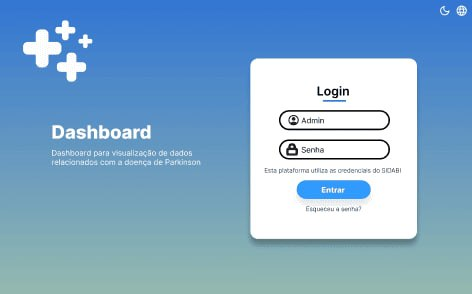
\includegraphics[width=0.8\textwidth]{telaInicial.jpeg}
    \centerline{\footnotesize Fonte: Elaborada pelos autores (2026).}
\end{figure}

A Figura~\ref{fig:telaInicial} apresenta a tela inicial de autenticação da aplicação \textit{desktop} do Painel Parkinson. Essa interface representa o primeiro contato do profissional da saúde com o sistema, sendo responsável pelo controle de acesso aos \textit{dashboards} clínicos e às informações relacionadas aos pacientes. 
A proposta visual da interface busca reduzir a complexidade de navegação inicial e permitir acesso rápido às funcionalidades do Painel Parkinson, contribuindo para uma experiência mais eficiente no contexto clínico. 

\subsection{Escolha de perspectiva}
\begin{figure}[H]
    \centering
    \caption{\textit{Dashboard} clínico do Painel Parkinson em ambiente\textit{desktop}.}
    \label{fig:dashboardClinico}
    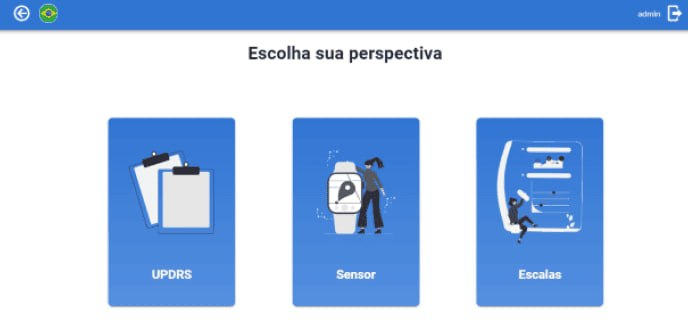
\includegraphics[width=0.8\textwidth]{dashboardClinico.jpeg}
    \centerline{\footnotesize Fonte: \cite{oliveira2023}}
\end{figure}

Após a autenticação no sistema, o usuário é direcionado para a tela de escolha de perspectiva da aplicação \textit{desktop} do Painel Parkinson, conforme apresentado na Figura 3.5. Essa interface tem como objetivo permitir o acesso aos módulos de visualização e análise disponíveis no sistema. Embora a interface base preveja a expansão arquitetural para múltiplos módulos, a presente versão do protótipo foca exclusivamente no acesso e análise da perspectiva \textit{Unified Parkinson's Disease Rating Scale} (MDS-UPDRS). A seleção deste módulo direciona o profissional da saúde para as informações clínicas, permitindo avaliar o estado motor e não motor do paciente de forma padronizada.

\subsection{Listagem de pacientes}

\begin{figure}[H]
    \centering
    \caption{\textit{Dashboard} clínico do Painel Parkinson em ambiente \textit{desktop}.}
    \label{fig:listagem}
    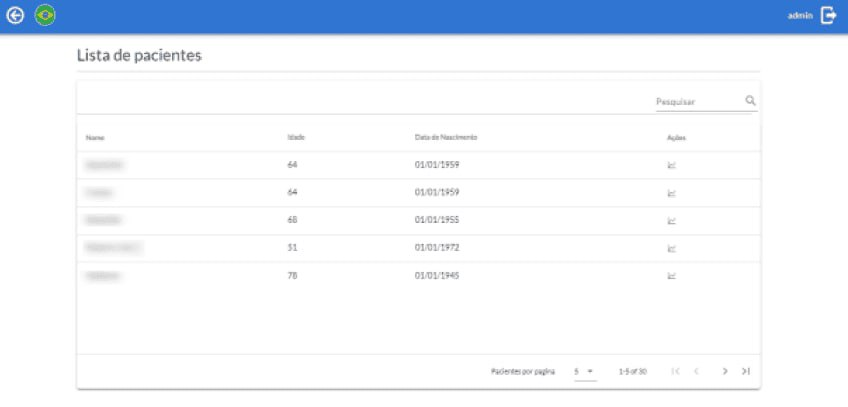
\includegraphics[width=0.8\textwidth]{listagem.jpeg}
    \centerline{\footnotesize Fonte: \cite{oliveira2023}}
\end{figure}

Após a seleção da perspectiva desejada, o usuário é direcionado para a tela de listagem de pacientes, conforme apresentado na Figura~\ref{fig:listagem}. Essa interface tem como principal objetivo organizar e disponibilizar os registros dos pacientes cadastrados no sistema, permitindo acesso rápido às informações clínicas e avaliações relacionadas à Doença de Parkinson.
A tela apresenta uma estrutura baseada em tabela, contendo informações como nome do paciente, idade e data de nascimento, além de funcionalidades de pesquisa e navegação entre registros. Essa organização busca facilitar a localização de pacientes específicos e otimizar o fluxo de utilização da aplicação no contexto clínico.
Além disso, a interface disponibiliza ações individuais para cada paciente listado, permitindo acesso aos \textit{dashboards} clínicos, gráficos e resultados das avaliações armazenadas no sistema. A proposta da tela visa reduzir a complexidade de navegação e melhorar a eficiência do acesso às informações durante o acompanhamento clínico. Além das funcionalidades de navegação, a aplicação realiza a sincronização automática dos dados clínicos em segundo plano (\textit{background}), mantendo as informações do paciente atualizadas durante a utilização do sistema. Esse mecanismo reduz a necessidade de intervenção do profissional de saúde para atualização dos registros, contribuindo para a disponibilidade contínua do histórico biomédico. Como medida de contingência, a aplicação poderá disponibilizar uma sincronização manual em situações excepcionais.

\subsection{\textit{Dashboard} clínico}

\begin{figure}[H]
    \centering
    \caption{\textit{Dashboard} clínico do paciente na perspectiva UPDRS.}
    \label{fig:perspectivaUPDRS}
    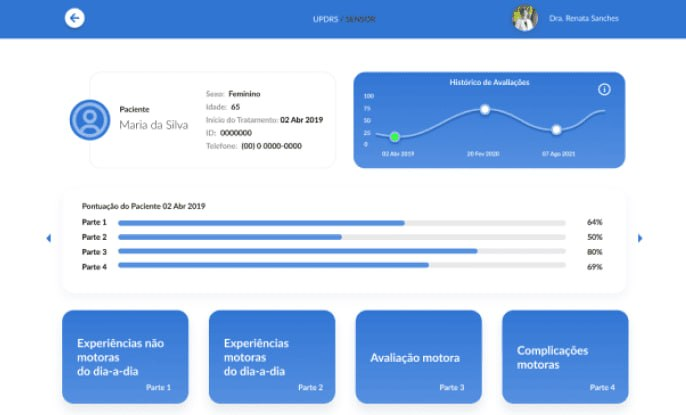
\includegraphics[width=0.8\textwidth]{perspectivaUPDRS.jpeg}
    \centerline{\footnotesize Fonte: \cite{oliveira2023}}
\end{figure}

Após a seleção do paciente na listagem principal, o sistema direciona o usuário para a tela de visualização clínica individual, conforme apresentado na Figura~\ref{fig:perspectivaUPDRS}. Essa interface representa o principal painel de acompanhamento do Painel Parkinson, reunindo informações relacionadas à evolução clínica do paciente.
A tela apresenta dados pessoais básicos do paciente, como nome, sexo, idade e informações relacionadas ao acompanhamento clínico. Além disso, o sistema disponibiliza um gráfico cronológico contendo o histórico das avaliações realizadas, permitindo a visualização da evolução dos resultados ao longo do tempo.
Os dados clínicos são organizados conforme a estrutura da escala \textit{Unified Parkinson’s Disease Rating Scale} (UPDRS), dividida em quatro partes principais: experiência não motora do dia a dia, experiência motora do dia a dia, avaliação motora e complicações motoras. Essa divisão permite que os profissionais da saúde realizem análises mais específicas sobre diferentes aspectos relacionados à Doença de Parkinson.
A organização visual dos gráficos e indicadores busca facilitar a interpretação das informações clínicas e contribuir para uma análise mais rápida e eficiente durante o acompanhamento dos pacientes. Dessa forma, o \textit{dashboard} clínico constitui uma das principais funcionalidades do sistema, atuando diretamente no suporte à decisão clínica.


\section{Testes e Análise Preliminar}
\label{sec:TestesAnalisepreliminar}

\subsection{Testes de Interface e Funcionamento Local}

Espera-se que a solução tecnológica desenvolvida possibilite a execução local, reduzindo a dependência de infraestrutura externa e entregando os benefícios operacionais previstos na concepção do software, como a eliminação da latência e a redução de custos de hospedagem.

A concepção dessa etapa avaliativa apoia-se nos princípios da Interação Humano-Computador (IHC). Segundo \cite{ihc2022}, a eficiência e a eficácia de um sistema computacional interativo estão diretamente ligadas ao seu tempo de resposta e à fluidez de navegação. Sendo assim, a avaliação do tempo de resposta, da estabilidade e da fluidez de navegação constitui parte importante da análise da adequação da ferramenta ao contexto de uso.

Para a realização prática dessa avaliação, a ferramenta será integrada ao fluxo de apresentações e uso de dados do grupo de pesquisa GPCA, conforme aprovação no comitê de ética CAAE nº 85830324.4.0000.5553, cujo material de divulgação consta no \hyperref[apendice:convite]{Apêndice \ref*{apendice:convite}}. Essa integração permite avaliar o desempenho do sistema em um cenário clínico padronizado pela linha de pesquisa institucional.

Como instrumento complementar para a avaliação da interação com a aplicação, será utilizado o questionário \textit{Health}, um instrumento padronizado e voltado especificamente para a avaliação da usabilidade percebida em sistemas de tecnologia em saúde. Após a realização das tarefas definidas no cenário de avaliação, os profissionais da saúde participantes responderão ao instrumento, permitindo obter uma medida quantitativa da percepção de facilidade de uso da solução. O resultado desta avaliação será utilizado como uma das métricas de validação da aplicação, em conjunto com as métricas técnicas obtidas durante os ensaios.

Durante esses ensaios, o foco da análise estará concentrado nas métricas técnicas e de resposta da solução \textit{desktop}, bem como na percepção de usabilidade dos profissionais participantes. Dessa forma, busca-se verificar o comportamento da aplicação quanto ao desempenho e à interação com o usuário no contexto proposto para suporte à decisão clínica.

O resultado desta avaliação será utilizado como uma das métricas de validação da aplicação, em conjunto com as métricas técnicas obtidas durante os ensaios, conforme detalhado a seguir.

\subsection{Instrumento de Avaliação de Usabilidade} 

A avaliação da usabilidade no contexto de Sistemas de Apoio à Decisão Clínica (SADC), como o Painel Parkinson Desktop, exige ferramentas metodológicas capazes de mensurar não apenas a interação superficial com a interface, mas também o impacto da tecnologia no fluxo de trabalho cognitivo e assistencial dos profissionais de saúde \cite{RussJara2025}. No âmbito do desenvolvimento da presente aplicação \textit{desktop} em Electron.js, voltada ao monitoramento longitudinal e à interpretação das escalas clínicas da Doença de Parkinson (como a MDS-UPDRS), a escolha do instrumento de avaliação deve estar rigorosamente alinhada aos objetivos clínicos e às especificidades dos especialistas que operacionalizam o sistema \cite{RussJara2025}. Nesse cenário, optou-se pela utilização do \textit{Health Information Technology Usability Evaluation Scale} (Health-ITUES) em detrimento de questionários de usabilidade genéricos, como o \textit{System Usability Scale} (SUS) \cite{RussJara2025}.

A justificativa metodológica para a preterição do SUS reside em suas limitações estruturais quando aplicado a tecnologias em saúde \cite{RussJara2025}. Embora o SUS seja amplamente disseminado na literatura geral, trata-se de uma escala unidimensional desenvolvida na década de 1980 para sistemas computacionais genéricos, contemplando apenas três dos dez atributos clássicos de usabilidade (aprendizagem, satisfação e facilidade de uso) e carecendo de itens voltados à utilidade clínica e à integração do sistema à prática médica \cite{RussJara2025}. Em contrapartida, o Health-ITUES é um questionário pós-teste de 20 itens concebido especificamente para a área de Tecnologia da Informação em Saúde (\textit{Health IT}) \cite{RussJara2025}. O diferencial do Health-ITUES consiste no fato de abranger todos os cinco atributos de usabilidade de Nielsen e Norman (eficiência, recuperação de erros, aprendizagem, memorabilidade e satisfação) e possuir um formato inerentemente customizável \cite{RussJara2025}. Essa flexibilidade permite adaptar a redação dos itens ao nome da aplicação (Painel Parkinson Desktop) e às tarefas clínicas específicas avaliadas (como a análise de pontuações da MDS-UPDRS), mantendo a validade de construto e permitindo comparações rigorosas entre diferentes fases de desenvolvimento do \textit{software} \cite{RussJara2025}.

A robustez psicométrica do Health-ITUES é amplamente sustentada na literatura recente de informática médica \cite{Gerchow2026}. Estudos de validação psicométrica demonstram que o instrumento apresenta elevada consistência interna, com alfa de Cronbach ($\alpha$) variando entre 0,79 e 0,96, além de forte validade de critério confirmada por correlações significativas com outras escalas consolidadas, como o PSSUQ \cite{Gerchow2026}. Adicionalmente, análises fatoriais exploratórias evidenciam uma estrutura conceitual sólida dividida em três fatores principais: Impacto e Utilidade Percebida, Facilidade de Uso Percebida e Controle do Usuário \cite{Gerchow2026}. Essas evidências comprovam a adequação e a sensibilidade do Health-ITUES para avaliar percepções de profissionais de saúde em ecossistemas digitais, garantindo um diagnóstico preciso da utilidade e do controle percebido durante o manuseio da ferramenta \cite{Gerchow2026}.

Do ponto de vista da aplicação prática em sistemas de apoio à decisão clínica e controle motor, o Health-ITUES consolidou-se como a ferramenta ideal e o padrão de referência em pesquisas recentes \cite{Tejeda2024}. Um estudo de caso aplicado ao desenvolvimento de um SADC para prevenção de quedas e prescrição de exercícios em idosos demonstrou a eficácia do Health-ITUES na avaliação com equipes de cuidados primários (médicos e assistentes), obtendo pontuações médias de usabilidade percebida de 4,5 (DP 0,8) em uma escala de 5 pontos e mediana de 5,0 \cite{Tejeda2024}. A sensibilidade do questionário permitiu mapear ganhos diretos na qualidade de vida de trabalho e na utilidade percebida, provando ser uma métrica sensível para quantificar como alertas e painéis decisórios auxiliam profissionais de saúde no manejo de condições motoras e de equilíbrio \cite{Tejeda2024}. Tal cenário guarda estrita simetria com o contexto do Painel Parkinson Desktop, onde o fluxo de trabalho dos especialistas (médicos, fisioterapeutas e terapeutas ocupacionais) depende da rápida interpretação de indicadores de motricidade e variabilidade de sintomas da Doença de Parkinson \cite{Tejeda2024}.

Dessa forma, para o protocolo de avaliação de usabilidade do Painel Parkinson Desktop, os 20 itens do Health-ITUES serão contextualizados para as tarefas de navegação nos \textit{dashboards} clínicos e exportação de laudos da escala MDS-UPDRS. O instrumento será aplicado de forma estruturada junto aos profissionais de saúde participantes após a realização dos cenários de teste simulados, mensurando quantitativamente as quatro subescalas do modelo: Qualidade de Vida no Trabalho, Utilidade Percebida, Facilidade de Uso Percebida e Controle do Usuário. Com essa fundamentação metodológica, assegura-se que a avaliação da migração para a arquitetura local em Electron produza evidências científicas válidas, de alta precisão e perfeitamente alinhadas aos padrões da informática em saúde.

\begin{quadro}[H]
    \centering
    \footnotesize
    \caption{Itens do Health-ITUES adaptados para a avaliação do Painel Parkinson Desktop.}
    \label{quadro:health_itues_itens}
    \begin{tabular}{|p{4cm}|p{10.5cm}|}
    \hline
    \textbf{Subescala} & \textbf{Item Adaptado ao Painel Parkinson Desktop} \\ \hline

    Qualidade de Vida\newline no Trabalho
    & 1. Acredito que o Painel Parkinson Desktop é uma adição positiva para o acompanhamento dos pacientes. \newline \vspace{0.15cm}
    2. O Painel Parkinson Desktop é uma ferramenta importante para a prática de monitoramento motor da Doença de Parkinson. \newline \vspace{0.15cm}
    3. O uso do Painel Parkinson Desktop melhora a qualidade das análises clínicas realizadas na instituição. \newline \vspace{0.15cm}
    4. O sistema otimiza o meu tempo de atendimento ao avaliar a progressão motora do paciente. \newline \vspace{0.15cm}
    5. A aplicação diminui o esforço manual necessário para o registro histórico e acompanhamento clínico. \\ \hline

    Utilidade\newline Percebida
    & 6. O uso do Painel Parkinson Desktop permite-me analisar as pontuações da MDS-UPDRS de forma mais rápida. \newline \vspace{0.15cm}
    7. O sistema aumenta a minha capacidade de identificar variações motoras e tremores nos pacientes. \newline \vspace{0.15cm}
    8. O Painel Parkinson Desktop facilita a geração e exportação de laudos e relatórios médicos em PDF. \newline \vspace{0.15cm}
    9. O recurso de exportação de dados anonimizados facilita a extração segura de informações para fins epidemiológicos. \newline \vspace{0.15cm}
    10. No geral, o Painel Parkinson Desktop é útil para o suporte à decisão clínica no acompanhamento da Doença de Parkinson. \\ \hline

    Facilidade de\newline Uso Percebida 
    & 11. A navegação entre os gráficos e os módulos do Painel Parkinson Desktop é clara e simples. \newline \vspace{0.15cm}
    12. É fácil aprender a operar a interface local do Painel Parkinson Desktop. \newline \vspace{0.15cm}
    13. Torno-me hábil rapidamente ao utilizar os filtros e gráficos do Painel Parkinson Desktop. \newline \vspace{0.15cm}
    14. A interface visual e os componentes de tela apresentam os dados biométricos de forma limpa e intuitiva. \newline \vspace{0.15cm}
    15. Recordo-me facilmente de como utilizar as funcionalidades da aplicação após um período sem uso. \\ \hline

    Controle do\newline Usuário
    & 16. Sempre que cometo um erro de navegação no Painel Parkinson Desktop, recupero-me de forma simples e rápida. \newline \vspace{0.15cm}
    17. Sinto que tenho controle total sobre a seleção de dados e exibição de parâmetros clínicos na tela. \newline \vspace{0.15cm}
    18. Consigo facilmente desfazer uma ação ou edição incorreta nos registros dos pacientes dentro do painel. \newline \vspace{0.15cm}
    19. O sistema fornece mensagens de confirmação e avisos claros ao realizar ações sensíveis de Alteração ou Exclusão. \newline \vspace{0.15cm}
    20. As respostas da aplicação às minhas ações na interface são previsíveis e consistentes. \\ \hline
    \end{tabular}
    
    \vspace{0.2cm}
    \centerline{\footnotesize Fonte: Elaborado pelos autores com base em \cite{RussJara2025, Tejeda2024}.}
\end{quadro}

\newpage %

A coleta de dados será realizada por meio de formulário estruturado aplicado imediatamente após a execução dos cenários de teste simulados \cite{Tejeda2024}. Cada item será avaliado em uma escala Likert de 5 pontos, variando de 1 (Discordo Totalmente) a 5 (Concordo Totalmente) \cite{Tejeda2024, Gerchow2026}. A análise quantitativa contemplará o cálculo das pontuações médias e medianas globais e por subescala, em que pontuações mais elevadas indicam maior usabilidade percebida \cite{Tejeda2024}. Adicionalmente, a consistência interna da amostra de profissionais de saúde será aferida pelo cálculo do Alfa de Cronbach ($\alpha$), assegurando a fiabilidade estatística dos resultados obtidos no contexto local \cite{Gerchow2026}.

\subsection{Métricas e Limiares de Validação}

\subsection{Resultados Esperados}

Espera-se que a solução tecnológica desenvolvida para o Painel Parkinson possibilite a execução local, reduzindo a dependência de infraestrutura externa e otimizando os recursos necessários para seu funcionamento. Pretende-se também verificar se a aplicação \textit{desktop} proporciona redução da latência no processamento e na renderização de dados clínicos, especialmente em operações que envolvam gráficos e informações biomédicas.

Espera-se, ainda, que a sincronização automática dos dados em segundo plano mantenha o histórico biomédico atualizado sem exigir intervenção constante dos profissionais de saúde. A avaliação da solução deverá contemplar também a percepção dos profissionais participantes quanto à facilidade de uso da aplicação, utilizando o questionário Health como instrumento padronizado de avaliação específico para o contexto clínico.

Por fim, pretende-se analisar o impacto do sistema desenvolvido sobre a redução dos custos operacionais relacionados à infraestrutura necessária para execução, além de verificar sua adequação ao contexto de suporte à decisão clínica. Os resultados obtidos deverão contribuir para identificar possíveis limitações da solução e estabelecer uma base para futuras evoluções do Painel Parkinson.